% title: An IR transform returns IR
% description: A transform consumes an IR and returns an IR that can be executed or transformed again.
\documentclass[tikz,border=5pt]{standalone}
\usetikzlibrary{arrows.meta}
\begin{document}
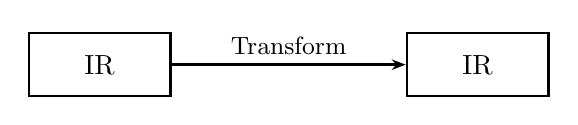
\begin{tikzpicture}[
    box/.style={draw, line width=0.8pt, minimum height=0.8cm,
                minimum width=1.8cm, align=center},
    flow/.style={-{Stealth[length=5pt]}, line width=0.9pt},
    note/.style={font=\small, align=center},
]

    \node[box] (in) at (0,0) {IR};
    \node[box] (out) at (4.8,0) {IR};
    \draw[flow] (in) -- node[note, above] {Transform} (out);

\end{tikzpicture}
\end{document}
